\documentclass[10pt]{article}
\usepackage[T1]{fontenc}
\usepackage[utf8]{inputenc}
\usepackage{lmodern}
\usepackage[a4paper,margin=24mm]{geometry}
\usepackage{amsmath,amssymb,booktabs,graphicx,array}
\usepackage{xcolor}
\definecolor{flm}{HTML}{A74C20}
\usepackage[colorlinks=true,linkcolor=flm,citecolor=flm,urlcolor=flm]{hyperref}
\usepackage{microtype}
\setlength{\parskip}{5pt}
\setlength{\parindent}{0pt}
\setlength{\emergencystretch}{2em}
\renewcommand{\arraystretch}{1.15}
\graphicspath{{figures/}}
\newcommand{\code}[1]{\texttt{\detokenize{#1}}}

\newcommand{\MatchedUpdate}{3000}
\newcommand{\BrowserUpdate}{3000}
\newcommand{\MatchedRows}{FLM & 600,003 & 1.9630 & 128.48 \\
GRU & 595,408 & 1.8913 & 107.58 \\
Transformer & 607,468 & 1.8870 & 106.45 \\}

\newcommand{\TestRows}{FLM & 1.9732 & 1.9756 & 1.9744 & 0.0017 \\
GRU & 1.9045 & 1.9052 & 1.9049 & 0.0005 \\
Transformer & 1.8770 & 1.8764 & 1.8767 & 0.0004 \\}
\newcommand{\NgramTest}{2.1208}
\newcommand{\TestIntervals}{42 & GRU & +0.0687 & [+0.0627, +0.0747] \\
42 & Transformer & +0.0962 & [+0.0891, +0.1024] \\
43 & GRU & +0.0704 & [+0.0655, +0.0750] \\
43 & Transformer & +0.0992 & [+0.0930, +0.1050] \\}

\hypersetup{pdftitle={FLM: A Fly-Wired Recurrent Language Model},pdfauthor={Kuber},pdfsubject={Working methods and validation report},pdflang={en}}
\title{\textbf{FLM: A Fly-Wired Recurrent Language Model}\\[6pt]\large An inspectable small-data experiment with matched lexical baselines}
\author{Kuber\\\href{https://flm.kuber.studio}{flm.kuber.studio}}
\date{10 September 2026 --- working research report}
\begin{document}
\maketitle
\begin{abstract}
We implement a compact language model whose directed recurrent topology is selected from a fruit-fly connectome. A differentiable rate core with fast and slow state receives a learned text interface and predicts a lossless, training-only byte-pair vocabulary. The 600,003-parameter model is compared with a 595,408-parameter GRU and a 607,468-parameter decoder transformer on the official WikiText-2 raw partitions. All models share lexical dimensions, training windows and update budgets. Across two completed training seeds, full test loss averages 1.9744 bits/byte for FLM, 1.9049 for GRU and 1.8767 for transformer. FLM outperforms a separate n-gram reference but trails both neural baselines. Acute interventions show that recurrence and slow state contribute to its learned predictions. The browser exposes actual state and a separate readout adapter. Verified 10M/100M-word BabyLM corpora and reproducible physical walking controls establish subsequent research stages; they do not establish a language-trained animal or a competitive general assistant.
\end{abstract}

\section{Question and scope}
Can an anatomical wiring constraint be a useful prior for language prediction under a small training budget? FLM makes this question concrete rather than treating a connectome as a pretrained intelligence. Training from scratch means that no learned language weights, pretrained embeddings, pretrained tokenizer or synthetic teacher corpus are imported. It does not mean absence of priors: graph selection, sign assumptions, pooling, nonlinearities and optimization all impose structure.

The intended contribution is an inspectable experimental system: reproducible graph and text acquisition, a compact recurrent architecture, matched baselines, exact browser parity, and visible separation between prediction, adaptation and body animation. A new name is not evidence of an algorithmic breakthrough. The current evidence supports a functioning next-token predictor and a testable architectural hypothesis, not a competitive general assistant.

\section{Research foundations}
MaleCNS provides anatomical connectivity and neuron identities \cite{malecns,google}. Simplified connectome-based dynamics have been used to investigate specific sensorimotor responses \cite{shiu}; task optimization within anatomical constraints has precedent in models of fly visual computation \cite{lappalainen}. Neither result licenses transfer of behavioral validity to a language-trained, central-brain subset with artificial interfaces.

Connectome-based reservoir computing is established prior work. Morra and colleagues studied a fly lateral-horn reservoir on a multifunctionality benchmark \cite{morra}. FLM differs from a fixed reservoir because it learns edge magnitudes and time constants as well as its input and readout. That difference must itself be evaluated; it is not inherently an improvement. Eligibility-trace learning provides another recurrent-learning direction \cite{bellec}, but FLM currently uses backpropagation through time, not a biological credit-assignment algorithm.

Transformers \cite{attention}, gated recurrent models \cite{gru}, SpikeGPT \cite{spikegpt}, RWKV \cite{rwkv} and Mamba \cite{mamba} establish that attention-free or recurrent language prediction is not new. FLM's narrow research question concerns this graph prior and these memory filters under declared conditions. Sparse connectivity alone does not establish lower power consumption on conventional hardware.

\section{Anatomy and graph construction}
The pinned source snapshot contains 166,700 annotated neurons, 25,582,938 directed neuron-pair edges and 124,177,617 contacts. These are counts of the acquired runtime representation, not a claim that the compact model contains the complete biological circuit. File sizes, hashes, index ranges, orientation and contact sums are independently checked. The snapshot is identified in the repository's source manifest.

The language core selects the 1,024 central-brain neurons with the largest incoming-plus-outgoing contact strength among the declared central intrinsic population, before inspecting language outcomes. Its induced graph retains 76,130 edges. Discarded boundary connections are absent; no unobserved external neurons are silently simulated. Type-ordered balanced pooling produces 128 pools. Five selected neurons lack finite soma coordinates and remain in inference but are omitted from positional rendering.

\begin{figure}[ht]
\centering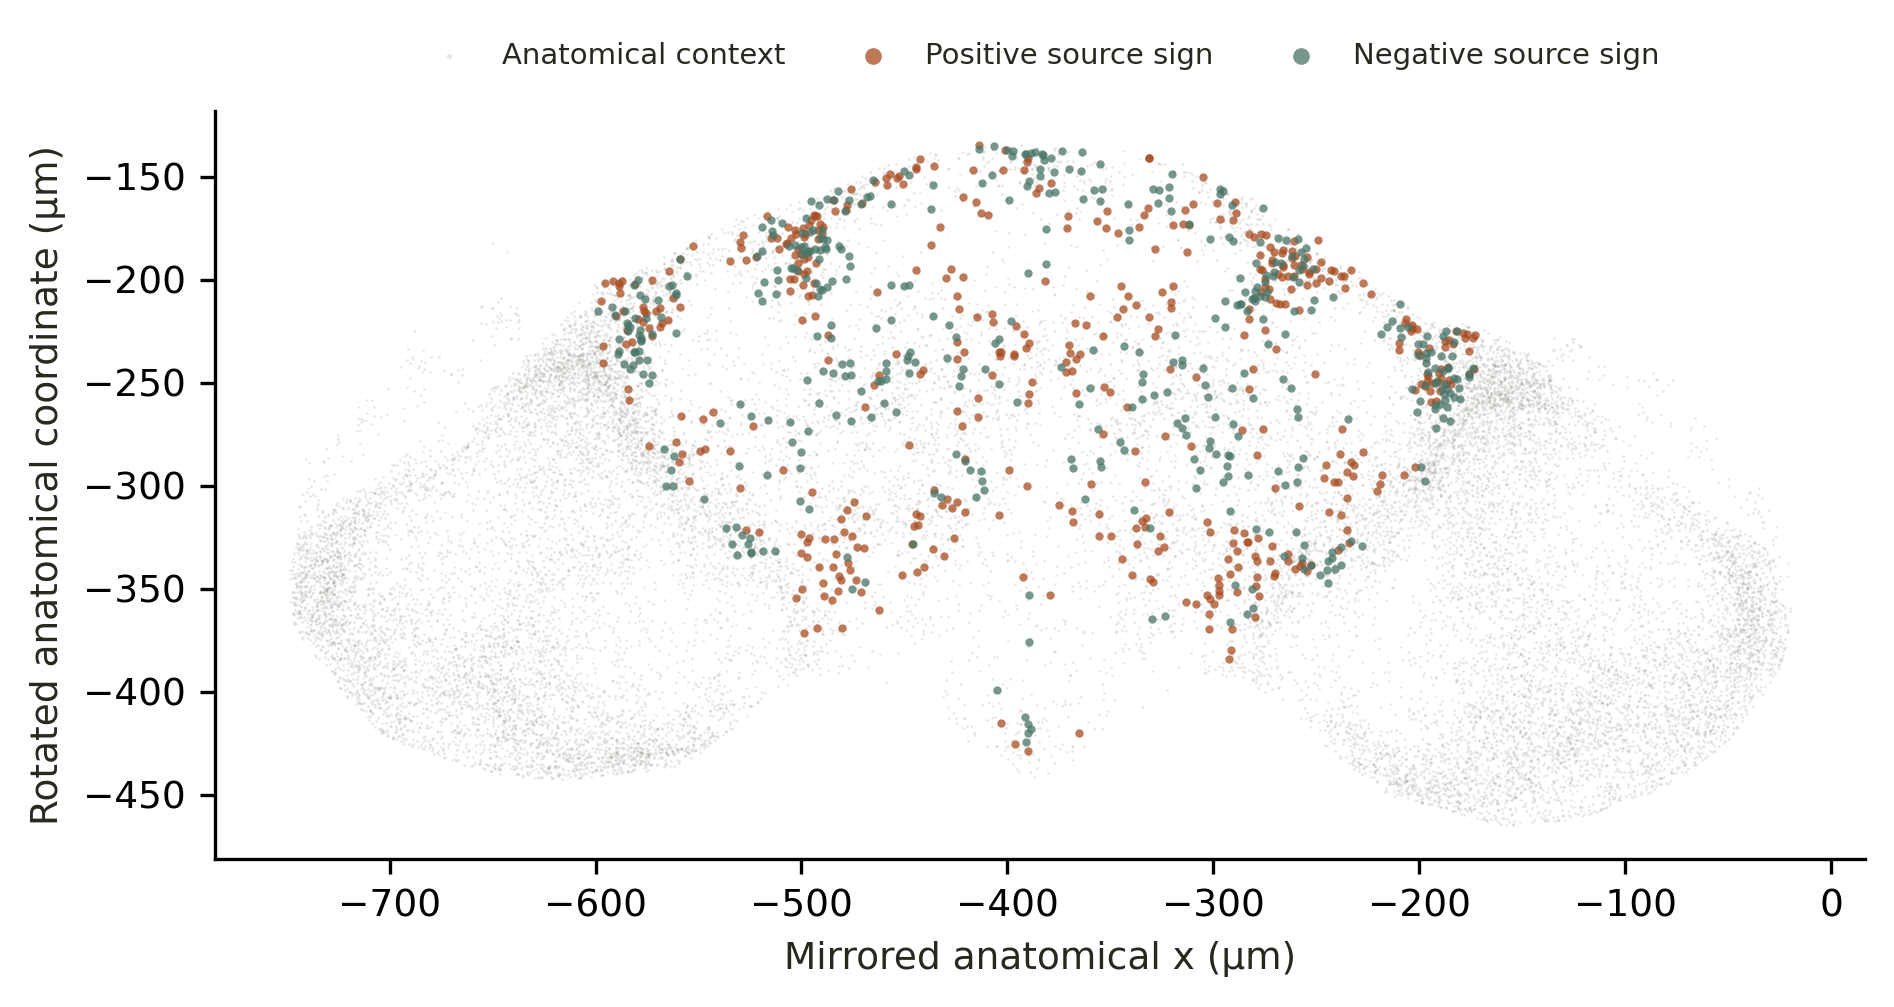
\includegraphics[width=.9\linewidth]{anatomy.png}
\caption{Anatomical positions of the selected neurons over downsampled brain context. Color denotes the assumed source sign, not activity. The displayed coordinates are rigidly rotated and mirrored for readability. The browser instead colors active neurons from actual inference state.}
\end{figure}

Signs are modeling assumptions associated with source neurotransmitter metadata. Contact counts are not measured functional weights. A conflict between an upstream model-card description and runtime metadata for modulatory transmitters is recorded; the declared runtime rule uses zero for those signs, and zero-sign outgoing edges are removed. The complete provenance and selection card are part of the reproducibility record.

\section{Architecture}
Let $x_t$ be a token ID, $E\in\mathbb{R}^{4096\times96}$ a trainable embedding, $h_t,s_t\in\mathbb{R}^{1024}$ the fast and slow states, and $P$ balanced mean pooling to 128 features. For retained edge $j\rightarrow i$, let $c_{ij}$ be its contact count and $\sigma_j$ its declared source sign. Define
\begin{align}
v_{ij}&=\sigma_j\log(1+c_{ij})\exp(\operatorname{clip}(\theta_{ij},-3,3)),\\
W_{ij}&=v_{ij}/\max\!\left(10^{-8},\sum_k|v_{ik}|\right).
\end{align}
Missing edges remain zero. Positive multiplicative gains preserve sign, and incoming absolute normalization is repeated after learning the gains. The update is
\begin{align}
u_t &= A E[x_t]+b+gWh_{t-1},\\
h_t &= (1-\alpha)\odot h_{t-1}+\alpha\odot\tanh(u_t),\\
s_t &= (1-\beta)\odot s_{t-1}+\beta\odot h_t,\\
f_t &= \operatorname{LN}([Ph_t;Ps_t]),\\
z_t &= Rf_t+r,\qquad \ell_t=Ez_t+q.
\end{align}
Layer normalization uses $\epsilon=10^{-5}$. Learned bounds are $g=0.05+2.95\operatorname{sigmoid}(\gamma)$, $\alpha_i=0.05+0.90\operatorname{sigmoid}(a_i)$, and $\beta_i=0.002+0.098\operatorname{sigmoid}(b_i)$. These are discrete token-update rates, not milliseconds or inferred membrane constants. The same embedding matrix receives gradients from input encoding and output scoring. There is no attention layer or direct input-to-logit bypass.

The state is causal and bounded by the leaky $\tanh$ dynamics from zero initialization. Bounded values do not guarantee long-context retention, a stable local Jacobian or a useful attractor. The slow filter adds a timescale, but its effective memory depends on recurrence, input and the learned readout. An isolated scalar filter with rate $r$ has half-life $\log(0.5)/\log(1-r)$; this is a descriptive filter property rather than a measured language-memory horizon.

\begin{figure}[ht]
\centering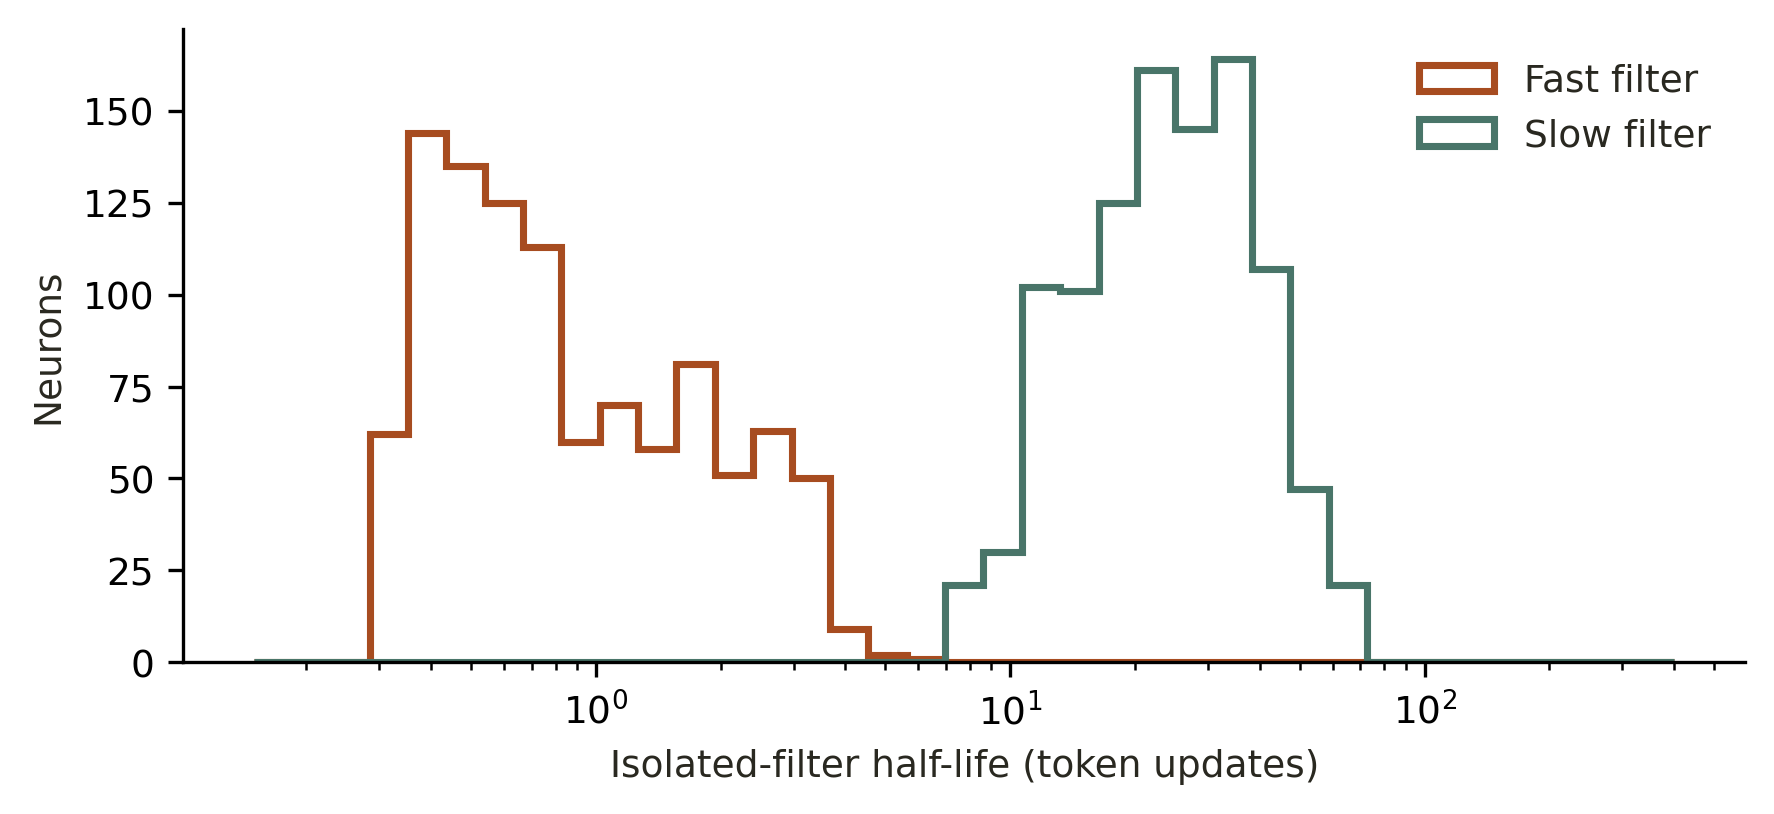
\includegraphics[width=.77\linewidth]{time-scales.png}
\caption{Learned isolated-filter half-lives at browser checkpoint \BrowserUpdate. Recurrent coupling and readout can change the effective task-level memory.}
\end{figure}

At this scale PyTorch uses a dense matrix containing the sparse pattern because it was faster on the available CPU. The browser uses destination-major compressed sparse rows and stores the tied embedding once, yielding a 2,713,236-byte inference-weight package. It computes input drives on demand instead of expanding all 4,096 tokens into 1,024-dimensional cached drives. Independent PyTorch fixtures verify logits, fast state, slow state and readout features.

\section{Data and matched evaluation}
WikiText was introduced to support language modeling with broader vocabulary and longer document structure \cite{wikitext}. We use the pinned raw variant, preserving official partitions of 600 training, 60 validation and 60 test articles. Training contains 2,051,910 whitespace-delimited words and 10,914,845 UTF-8 bytes. The raw variant still contains preprocessing artifacts such as punctuation markers; it is not an untouched Wikipedia dump.

A lossless byte-level BPE tokenizer is trained exclusively on the 600 training articles. It retains every byte through a complete byte alphabet and uses 4,094 text IDs plus explicit BOS=0 and EOS=1. No string in ordinary input is automatically treated as a boundary token. Training text averages 3.54 bytes per content token. Official split preservation, exact text reconstruction, hashes and limitations are detailed in the companion data note.

\begin{table}[ht]\centering
\begin{tabular}{lrl}\toprule
Model & Parameters & Core configuration\\\midrule
FLM & 600,003 & 1,024 neurons, 128 pools, two states\\
GRU & 595,408 & One layer, hidden width 200\\
Transformer & 607,468 & Two layers, width 108, six heads\\\bottomrule
\end{tabular}
\caption{All models share a 96-dimensional tied lexical interface and the same 4,096-token vocabulary. Each baseline is within 1.3\% of FLM's parameter count.}
\end{table}

The transformer has pre-normalized residual blocks, feedforward width 216, GELU and rotary positions; causal attention retains a 96-position window per layer. Streaming uses native bounded key/value caches, not repeated rescoring of the input prefix. The GRU uses its native recurrent hidden state. Their architecture-specific initialization remains part of the comparison and is recorded in source.

Each run uses 6,000 AdamW updates, batch 16 and sequences of 96 tokens. The first 16 positions warm the state and are excluded from the training loss. Sequences stay within articles. Training samples windows with replacement using a NumPy RNG independent of model initialization, so models with the same seed see identical inputs. Each run presents 9,216,000 input tokens. The learning rate warms up over 100 updates to 0.002 and decays by cosine to 0.0002; weight decay is 0.01 and gradient norm is clipped at 1.0. There is no dropout. Seeds 42 and 43 are registered for each main architecture.

Every 500 updates, validation uses deterministic per-article prefixes with a total quota of 32,768 target positions. State resets between articles and is carried within them. Boundary IDs are excluded from scored text. Selection minimizes validation bits per original UTF-8 byte:
\begin{equation}
\operatorname{BPB}=\frac{-\sum_{t\in\mathcal T}\log p(x_t\mid x_{<t})}{\log 2\;\sum_{t\in\mathcal T}\operatorname{bytes}(x_t)}.
\end{equation}
This measures the codelength of the canonical token sequence per byte. Shared-tokenizer perplexity is also reported; it must not be compared directly to published word-token WikiText perplexities. The same exact article bytes are required for paired final-test comparisons.

\section{Language results}
All six registered runs completed 6,000 updates. The first table reports matched seed-42 validation prefixes; the following test comparison uses the separately frozen validation-selected checkpoints. Every selected checkpoint came from update 6,000. Graph-specific superiority cannot be inferred without matched, retrained topology controls.

\begin{table}[ht]\centering
\begin{tabular}{lrrr}\toprule
Model & Parameters & Bits/byte & Token perplexity\\\midrule
\MatchedRows
\bottomrule\end{tabular}
\caption{Matched validation at \MatchedUpdate\ updates, seed 42. Lower is better. Values are generated directly from versioned evaluation artifacts.}
\end{table}
\begin{figure}[ht]\centering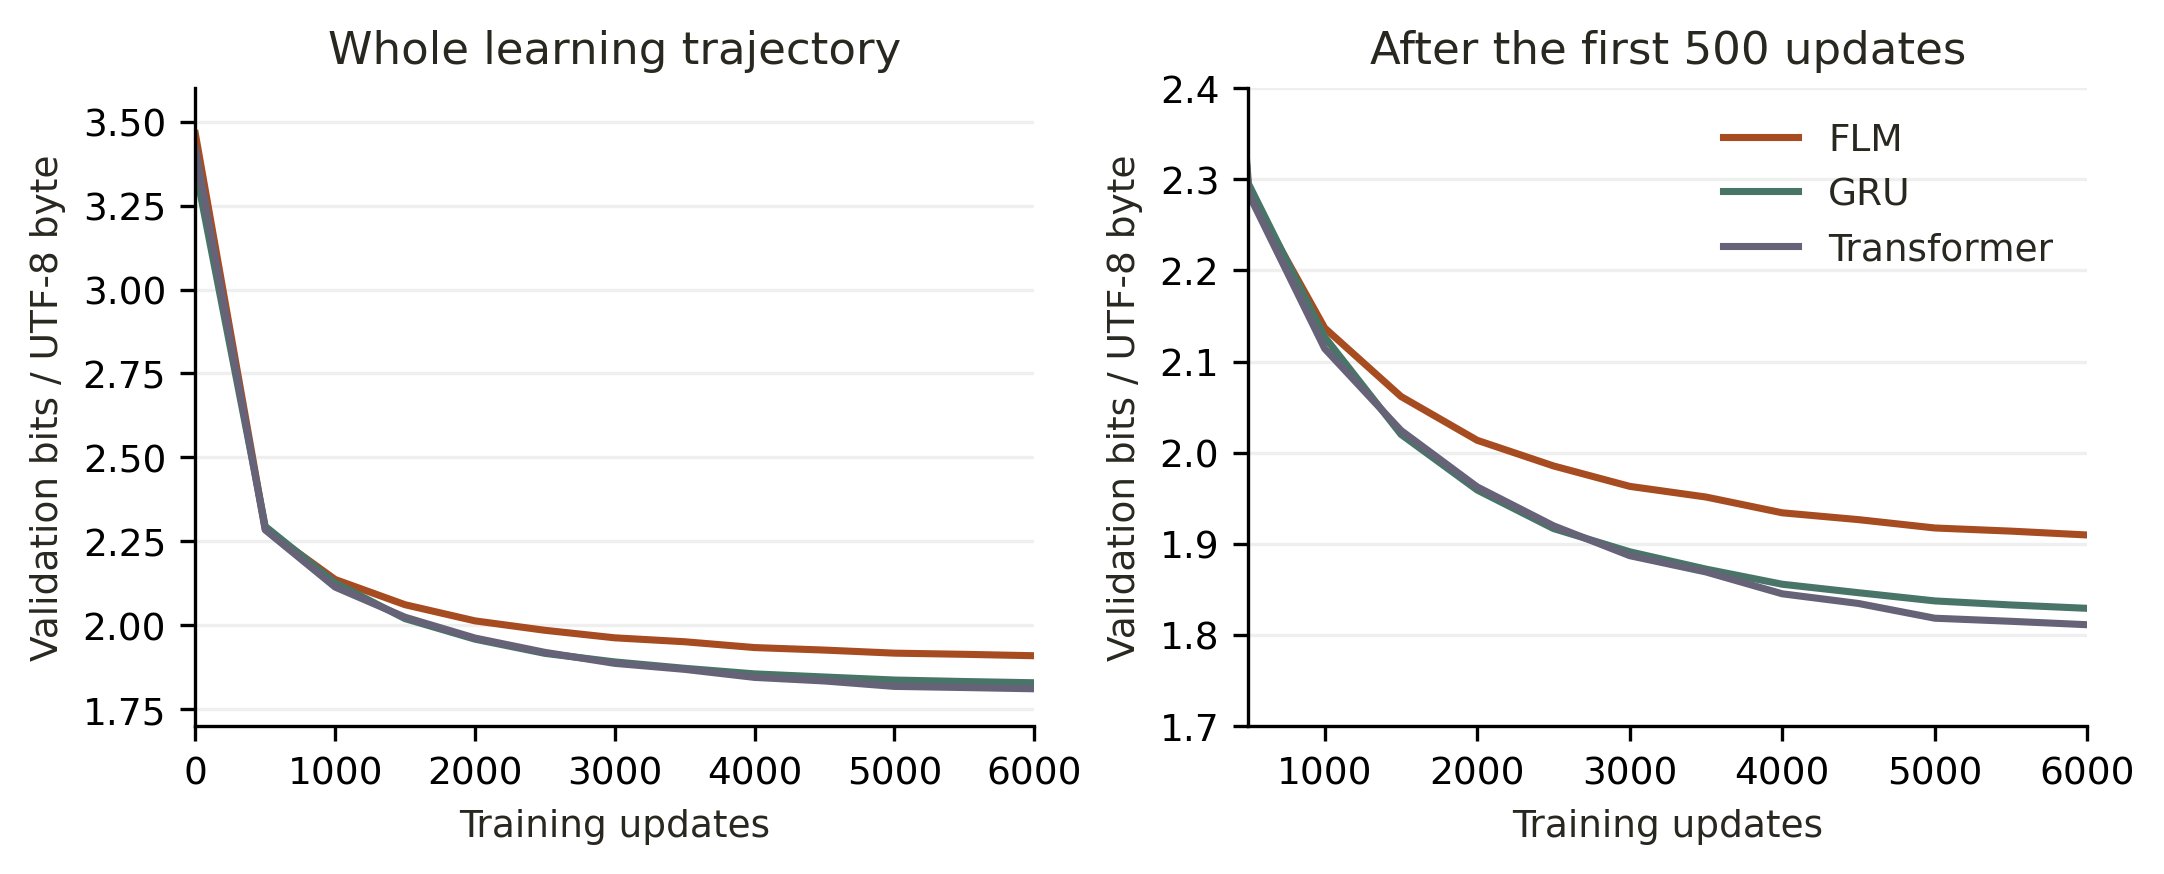
\includegraphics[width=\linewidth]{validation.png}
\caption{Completed seed-42 validation trajectories under the same update budget. The focused panel makes differences after early vocabulary acquisition visible.}\end{figure}

After freezing all six checkpoint hashes and the validation-selected n-gram smoothing, the complete 60-article test partition was scored: 367,981 text tokens and 1,287,656 UTF-8 bytes. Neither test loss nor generated samples determined checkpoint selection.
\begin{table}[ht]\centering
\begin{tabular}{lrrrr}\toprule
Model & Seed 42 & Seed 43 & Mean & Seed SD\\\midrule
\TestRows
\bottomrule\end{tabular}
\caption{Complete held-out WikiText-2 test loss, bits per UTF-8 byte. Lower is better. SD is the sample standard deviation of two training seeds.}
\end{table}
The separate four-byte-context n-gram scores \NgramTest\ bits/byte. FLM's mean loss is 0.0695 bits/byte above GRU and 0.0977 above transformer. Paired article resampling preserves a common byte denominator and yields positive FLM-minus-baseline intervals in both seeds.
\begin{table}[ht]\centering
\begin{tabular}{rlrr}\toprule
Seed & Baseline & FLM minus baseline & 95\% article interval\\\midrule
\TestIntervals
\bottomrule\end{tabular}
\caption{10,000 paired article bootstrap replicates. These intervals condition on the trained checkpoints; they do not include uncertainty from other corpora or architecture tuning.}
\end{table}

The current FLM result trails the conventional baselines. Unedited same-prompt continuations show learned word and phrase structure, but also repetition, malformed names, preprocessing markers and unsupported statements. These outputs justify completion mode rather than an assistant claim. A few attractive continuations would not demonstrate factual knowledge or understanding.

The earlier AMI byte experiment provides a separate negative result: at 6,000 updates FLM obtained 1.9683 validation-prefix bits/byte, while a smoothed four-byte-context n-gram obtained 1.6091 on its corresponding byte-prefix protocol. AMI and WikiText scores describe different distributions and tokenization protocols and must not be placed on one quality leaderboard. The n-gram is not parameter-matched.

\section{Memory, adaptation and visible behavior}
FLM stores 2,048 float32 state values, or 8,192 bytes per sequence. The GRU's hidden state is smaller at 800 bytes. The declared transformer's two-layer cache retains up to 95 past positions per layer and stores 164,160 float32 key/value bytes, excluding its scalar position counter. These calculations exclude weights, temporary activations, allocator overhead and adaptation. They are memory accounting, not speed or energy benchmarks.

\begin{figure}[ht]\centering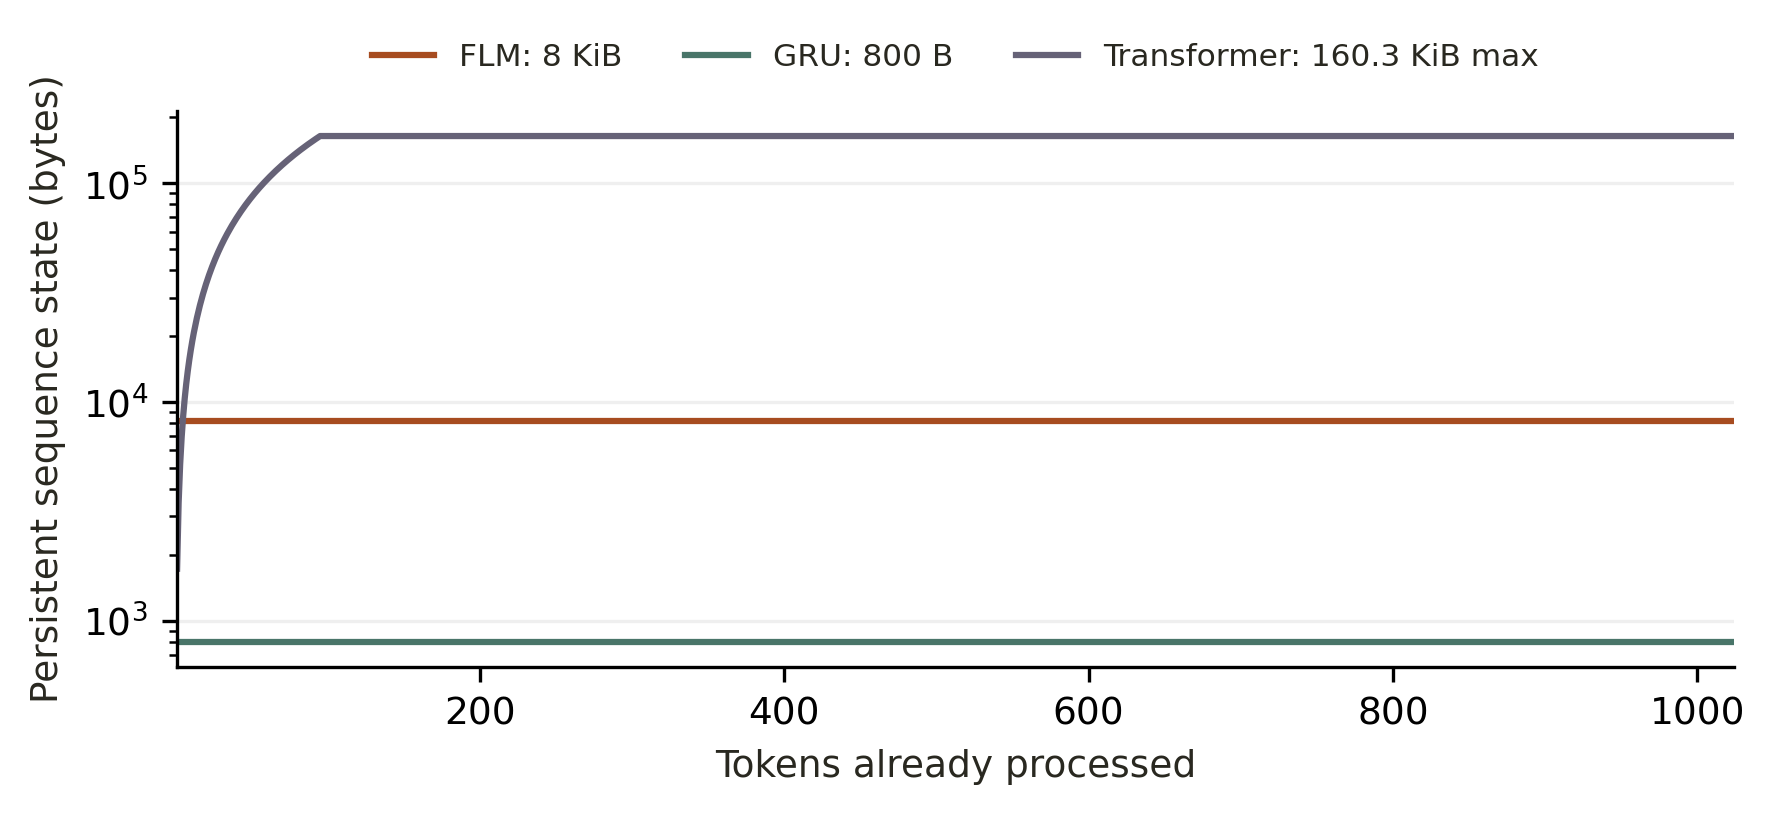
\includegraphics[width=.83\linewidth]{state-memory.png}
\caption{Persistent sequence-state storage derived from the implemented dimensions. The transformer's cache is bounded; FLM is not the smallest-state comparator.}\end{figure}

After training and preprocessing processes exited, an isolated four-thread float32 CPU measurement used the same 128-token prefix and 128 forced continuation tokens, one warmup and five repeats. Median prefill/decode rates were 4,060/200 tokens/s for FLM, 10,718/3,491 for GRU and 30,857/724 for transformer. Tokenization was excluded. The eager FLM path prepares recurrent weights at each forward call, including each one-token decode call; these timings describe this implementation and are not optimal-kernel, energy or hardware-independent comparisons. Measured owned state storage agrees with the dimensional accounting above.

Browser learning updates a separate $4096\times96$ output correction and bias by the observed next-token cross-entropy gradient, with rate scaling by $1/\sqrt{96}$, small decay and bounded coefficients. It does not modify the bundled embedding, recurrent wiring or time constants. Consequently, a fixed input has the same recurrent activity before and after readout adaptation; free generation can follow a different trajectory because its selected input tokens change. Separate probe text is scored before and after updates. Lower training loss alone may be memorization.

The 3D brain displays actual fast or slow state for modeled neurons. Gray points are anatomical context without simulated activity. Silencing a neuron zeroes both its states, and controls replay the same input from zero for an interpretable intervention. The body uses 39 attributed NeuroMechFly meshes and verified articulated kinematics \cite{neuromechfly}. It is a female body paired with a male brain graph. Head and wing offsets are designed summaries of state, not trained motor outputs, physics, reward learning or animal behavior.

\section{Mechanisms and physical controls}
Acute validation interventions remove recurrent inter-neuron communication or the slow-state feature without retraining. For seed 42, loss rises from 1.9097 to 2.0631 and 1.9952 respectively; for seed 43, it rises from 1.9107 to 2.0294 and 1.9899. Leak memory remains in the recurrence-off condition. Both trained models use these mechanisms, but disrupting a learned computation is not a matched architectural comparison. Replaying an original 77-token paragraph from zero state before and after training also gives different fast and slow trajectories.
\begin{figure}[ht]\centering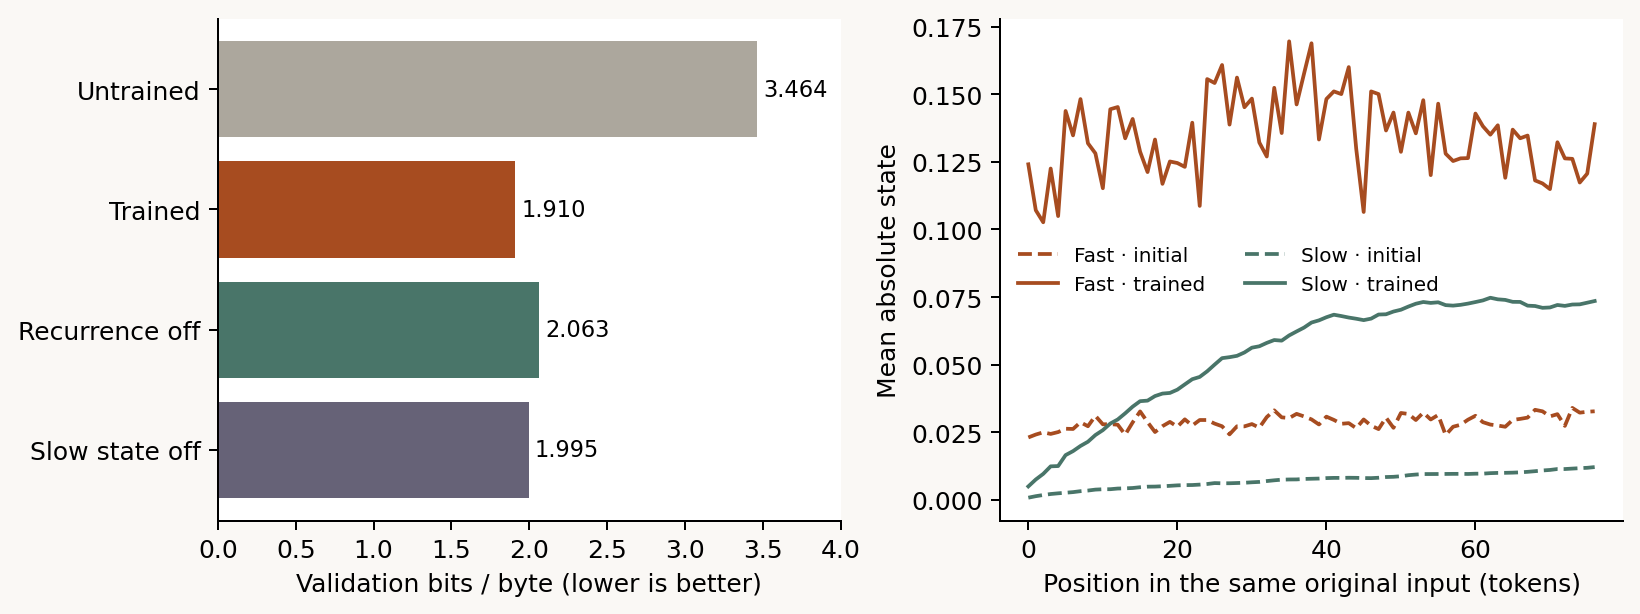
\includegraphics[width=\linewidth]{mechanism-s42.png}
\caption{Seed-42 validation interventions and responses to identical input. State magnitudes are measured, not animation signals. The diagnostic uses no test text.}\end{figure}

A separate Python 3.12 environment pins FlyGym 2.1.0 and MuJoCo 3.9.0 for actual articulated physics. A designed hybrid turning controller uses preprogrammed steps and contact feedback for 42 actuated joint degrees of freedom. After identical initialization and settling, one-second trials at 0.1 ms steps produce x displacement 13.461 mm under symmetric drive, and heading changes of $-2.556$ and $+2.811$ radians under opposite drive asymmetries. Repeating the symmetric trial reproduces every recorded thorax position exactly. All trajectories retain finite state and remain upright over this short calibration.
\begin{figure}[ht]\centering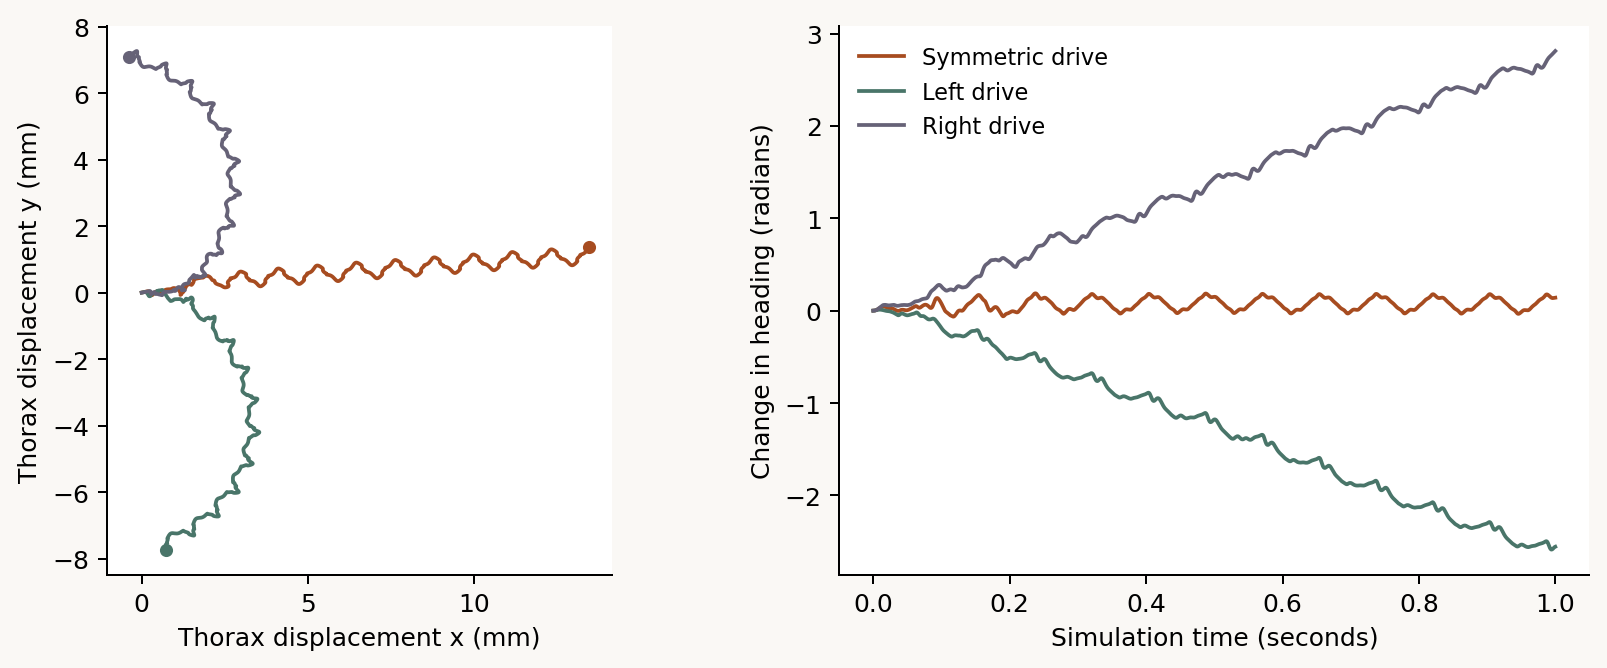
\includegraphics[width=\linewidth]{physical-calibration.png}
\caption{Measured physical trajectories and heading changes under prescribed descending drives. FLM is disconnected; no motor learning occurs in these controls. The associated recording is shown at quarter speed on the research page.}\end{figure}
This establishes a measurable action interface for future comparisons of fixed, language-trained and task-adapted recurrent cores. It is separate from the browser's illustrative pose mapping. Sensor observations, learned motor heads, rewards and task success must be recorded before claiming a learned skill or transfer from language.

\section{Limits and next experiments}
The selected central subset changes connectivity and removes biological inputs. Source signs, artificial pooling and rate dynamics simplify biology. The shared vocabulary, short training chunks, modest exposure and two seeds limit language and statistical conclusions. A CPU-friendly implementation may have very different cost on sparse accelerators. No energy efficiency or full-connectome training result is claimed.

The completed test intervals are conditional on trained checkpoints; two seeds do not characterize broad training variability. Follow-up controls preserve directed degrees and source-sign constraints through actual edge rewiring, and retrain disabled-mechanism models under the same schedule before attributing a benefit to anatomy.

The next registered language study uses verified BabyLM 2026 10M/100M-word corpora and a shared tokenizer fitted to the 10M training set, as detailed in the data note. A fixed 6,700-pair BLiMP diagnostic panel \cite{blimp} adds grammatical contrasts beyond average likelihood; it is evaluation-only, not a synthetic training corpus. Longer-term studies compare delayed recall, interference, adaptation retention and forward-time eligibility or reward-modulated learning against BPTT. Such learning rules have prior work and are not unique to fly wiring. Whole-graph training remains a separate capacity and kernel study. The empirical direction must follow measured improvements and failures rather than the assumption that anatomy guarantees an advantage.

\begingroup\raggedright
\bibliographystyle{plain}
\bibliography{references}
\endgroup
\end{document}
